% -*- mode: LaTeX -*-
% -*- mode: LaTeX; tex-command: "pdflatex" -*-

% $Id$
%
% Log at the end.
%
% Text in \textsf{###} is ``to be checked''.  No fields must be left
% in such a tag when the report is finished.


\documentclass[draft,a4paper]{article}

%\usepackage{concrete}          % ok - legible
%\usepackage{beton}             % ok - legible
%\usepackage{times}             % ok - standard
%\usepackage{utopia}            % ok
\usepackage{charter}            % ok - very legible, good in PDF
%\usepackage{bookman}           % ok - legible
%\usepackage{helvetic}          % no change
%\usepackage{palatino}          % ok - nice, like it
%\usepackage{lucidabr}          % No good, due to missing fonts here.
%\usepackage{a4wide}
\usepackage{fullpage}
\usepackage{isolatin1}
%\usepackage{parskip}
% \usepackage{draft}
\usepackage{verbatim}
\usepackage{graphicx}
\usepackage[%pdftex,
  pdftitle={Database backed Websites},
  pdfauthor={Thorbjoern Ravn Andersen},
  pdfsubject={pdfsubject},
  pdfkeywords={pdfkeywords},
  pdfpagemode={UseOutlines},
  bookmarks,bookmarksopen,
  pdfstartview={FitH},
  colorlinks,linkcolor={blue},citecolor={blue},
  urlcolor={red}
]{hyperref}

%%%%%%%%%%%%%%%%%%%%%%%%%%%%%%%%%%%%%%%%%%%%%%%%%%%%%%%%%%%%
%
% new commands
%
% \framepage{15cm}{text}
\newcommand{\framepage}[2]{\begin{center}\fbox{\begin{minipage}{#1}#2
      \end{minipage}}\end{center}}

% \unixcommand{emacs}
\newcommand{\unixcommand}[1]{``\texttt{{#1}}''}
% \ntcommand{jview}
\newcommand{\ntcommand}[1]{``\texttt{{#1}}''}

% \myurl{http://sunsite.auc.dk}{The Danish SunSite}
\newcommand{\myurl}[2]{\begin{underline}{#2}\end{underline}\footnote{{#1}}}

% \tag{hr}  ->  <hr>
\newcommand{\tag}[1]{$<$#1$>$}

%%%%%%%%%%%%%%%%%%%%%%%%%%%%%%%%%%%%%%%%%%%%%%%%%%%%%%%%%%%%

\author{ Thorbj{\o}rn Ravn Andersen}

\title{Database backed Websites \\
  \textit{D R A F T -- $ $Revision$ $}} % Math hack for RCS

\bibliographystyle{alpha}

\begin{document}
\maketitle

\begin{abstract}
  This thesis discusses database backed websites; their current use as
  presentation engines, construction, pros and cons, list the current
  state of the art software, and how web sites in general function as
  \textit{information presenters}.  Hereafter it is discussed how
  end-users best can utilize such a system, without giving up their
  current software, allowing such websites to be used to ease the
  distribution of information between users, and let the web site
  provide \textit{information sharing}.
  
  Technologies are discussed with an emphasis on Open Source software,
  and two sample programs - ``Cactus'' and ``Consensus'' are
  presented,  and discussed.  Cactus allows any user to do automated
  SSP on an Intranet without a human webmaster to convert documents
  and maintain links.  Consensus allows an open group of people to
  maintain a set of documents on a webserver.
  
\end{abstract}
Stuff to place:  Java has unicode support, multithreads.


\textbf{Note: }Framed text is unexpanded keywords which eventually
will be replaced with prose.

\section{What is a database backed webserver?}

A \textit{databased backed webserver} is a webserver which has access
to a database at the same time as it serves documents to clients.
Such access opens new possibilities, some of which are:

\begin{itemize}
\item The database can protect against race conditions when data is
  updated on the server.
\item Provide a searching facility more complex than grep.
\item Allow fast access to data without worrying about limitations in
  file systems
\item ``\textsf{users can extract data on their own if they want to}''
\item Databases are optimized for disk I/O, webservers for network
  I/O.  Those go well together.
\item Very large amount of data can be online
\item Data can be managed remotely by others than the webmaster
\item \textsf{what else?}
\end{itemize}


\subsection{Protection against race conditions}
\label{sec:protection-against-race-conditions}

A database can provide atomic operations on its data, as opposed to a
stock Unix file system, where data unwittingly can be corrupted if two
processes try to read and update information at the same time.  The
concept is well known from multi-programming \textsf{the eskimo book?}

Companies like ``valueclick'' and ``\textsf{doubleclick?}'' sell
banner ad's (the \textsf{480x120?} pixel advertisements allowing you
to click through to the advertisors website if you are interested).
These are either sold by the number of \textit{impressions} (shown to a
user) or \textit{clicks} (where the user actually clicks on the
banner), and these must be counted in order to document that the
customer gets what he pays for, and the banner ad provider does not
expose more than what the customer paid for.

Here is a database system essential in order to protect the data from
being accidentially overwritten.  ValueClick states that they have
\textsf{7 million impressions}  daily, which is around 80
impressions pr second.

\textsf{And what else is new?}

\subsection{Provide searching facilities}
\label{sec:providing-searching-facilities}

A flat file basically only allow you to search the content and the
filename with modifications based on the timestamps of the file.
Searchings normally happen linearly through files and directories.

Since a database may have a lot more attributes, queries can be much
more sophisticated, and may even be done against indexed data.

\subsection{Allow fast access to data without using file systems}
\label{sec:allow-fast-access-to-data}



\subsection{????}



\subsection{Databases are optimized for disk I/O, webservers for network}
  I/O.  Those go well together.
\subsection{Very large amount of data can be online}
\subsection{Data can be managed remotely by others than the webmaster}
\subsection{Others?}


\framepage{15cm}{
Provide background information: Quick overview of the technology
[webserver, database, http, sql, dynamically generated content vs]
with a graph.  Give simple example.  Explain \textsl{when} things
happen (on-the-fly vs statically generated pages).  Explain the
advantages and disadvantages databases have over flat filesystems
[transactions(protection, atomicity), extra attributes, speed, indexed
columns, complex queries, scalability(linear search in filesystems,
multihost db's),}

\section{The new role of the webserver}

\framepage{15cm}{
Compare original functionality with static HTML-files with content and
a few CGI-scripts, to the current dynamically generated sites with
many hits pr day.  Since HTML is generated and provides little
abstraction it is hard to use on a higher abstraction level, and with
unreadable code in ASP and PHP3 it is harder.  CSS was not the answer
since it did not provide any abstraction from the presentation
(seperate content from layout).

Different needs of the user - wap/pdf/html/braille.  CPU, storage,
webmaster time prevents all formats being pregenerated.
}


% \section{Terms and concepts}
% \framepage{15cm}{
% Explain XML, XSL, XSLT, HTML (yes!), SQL, SAX, DOM, XSP and whatever
% fancy terms come to mind.  Draw graph of what happens with an XML
% document.}
% $Id$

\chapter{Terms and concepts}
%\section{Terms and concepts}
\label{cha:terms-and-concepts}

\mycitation{``HTML is a SGML DTD''}{\textsf{?}}{\textsf{?}}


This report uses a lot of abbreviations, many of which may not be
widely known.  This section lists mosts of them.


\textsf{The list will be sorted}
\begin{description}

\item[entity] A named ``unit'' in XML/SGML which expands to a string.
  This is very similar to a macro without arguments in other
  languages.
  
\item[XSL-FO] XSL-formatting objects.  A generic description of the physical
  layout of a XML-document on paper.  These files can be converted to
  PDF with FOP or PassiveTeX
  
\item[SGML] A family of languages.  The \textit{DTD} specifies which
  language it is.  SGML can be formatted with FOSI or DSSSL
  style-sheets.  \unixcommand{jade} can format to HTML, plain text and
  RTF. 
  
\item[XML]
% A family of languages.  The \textit{DTD} specifies which
%   language it is.  XML-documents can be transformed with
%   \textit{XSL}-style sheets to another XML-document (this process is
%   called \textit{XSLT}).  XML is a subset of \textit{SGML}
  
XML is a light-weight version of SGML (both defines document
languages) designed to be embeddable in a browser.  XML-documents
\textit{may} comply to a DTD, or be stand-alone (``DTD-less'').  XSL
is used to convert a XML document into another XML document (XSLT) or
into the generic page description language XSL-Formatting Objects
(XSLFO).


\item[*ML] Common description of both XML and SGML, where the two have
  the same applications.

\item[DTD] The \textsf{Document T? Description} is the specification
  which describes the exact syntax of the *XML


\item[XSLT] Either the process of \textit{transforming} a XML-document into
  another XML-document using a XSL-stylesheet, or the process of
  \textit{formatting} a document into FO, which then can be further
  formatted in PDF.

\item[DOM] \textsf{W3C's initial model for representing an XML tree
    internally.  Superceeded by SAX (\textsf{for java?)}}
  
\item[SAX] Simple Application \textsf{interface for?} XML.  An event
  based approach to XML-parsing and representation.  Has an advantage
  in that the design allows processing to begin before the whole
  XML-tree has been read in.  (\textsf{URL?}).  Parsers and
  \textsf{processors?} which implement SAX can be selected freely,
  currently allowing for \textsf{20 different combinations of parsers
    and whashallicallem}.


\item[HTML] Hyper Text Markup Language.  The ``language of the web''
  which was originally designed by a physicist to present articles to
  other physicists.  Was later hacked upon by Netscape and Microsoft
  to do things it was never originally meant to do.

  
\item[DSSSL] \textsf{SGML style sheets something}.  Is used to render
  an SGML document to another format.  \unixcommand{jade} can render
  to \textsf{FOT}, RTF, {\TeX} (must be post-processed with
  \unixcommand{jadetex}), SGML and XML.  \textsf{Is this a standard?}
  
\item[FOSI]  \textsf{Another style sheet for SGML}, which I do
  not know anything about.  Apparently the US Navy uses it a lot.
\textsf{  Check in DocBook.}

  
\item[SQL] The Structured Query Language is the \textsf{standard}
  language for communicating with a database.

  
\item[XSP] \texttt{XML Servlet Pages} - A technique for combining code
  with XML in a single page, which is parsed and executed by the
  webserver when it is requested.

\item[RTF] \textit{Rich Text Format} - a document description language
\textsf{designed by microsoft}.  Widely supported.  May contain
extensions to the original RTF-specification.

\item[Jade] A DSSSL-engine for SGML documents by James Clark.

\item[JPEG] An efficient method for representing photographs in
  computer files.  Efficiency is achieved by discarding parts of the
  visual information which is hardest for the human eye to see.
\item[GIF] An image format well suited for computer generated images
  with few distinct colors, like icons.  Is hampered by a patent on
  the compression scheme used and a maximum of 256 colors.
  Superceeded by PNG.
\item[PNG] The successor to GIF.  Is supported in newer browsers
  only.  
\item[CGI] The Common Gateway Interface.  The original way to generate
  pages and other files dynamically.  A CGI-script can be written in
  any language supported by the web server.

\item[IIS] Microsoft Internet Information Server.  The webserver from
  Microsoft. 
  
\item[ftp] File Transfer Protocol.  This is both the name of the
  \textit{protocol} (the method) as well as the \textit{program}
  implementing the protocol.  ftp can transfer files between a client
  computer and a server computer, and is a standard on the Internet
  
\item[http] Hyper Text Transfer Protocol.  This is the protocol a web
  browser needs to speak with a web server, in order to retrieve
  documents.  Http is intentionally very simple.
\item[TCP/IP] This is the procotol which a computer needs to speak to
  connect to the Internet.  It allows two computer to establish a data
  stream, where one machine pushes bytes in one end of the stream, and
  the other machine retrieves the bytes from the other end of the
  stream, without either computer being concerned about the underlying
  network. 
\item[SP] A \textsf{what}?
\item[Perl] A scripting language which has become popular with Unix
  system administrators, and which ``was there'' when a need for
  scripting languages for CGI arose.  Has eminent regular expressions.
\item[ASP] Microsofts version of a scripting language intertwined with
  HTML. Works on Microsoft web servers only.
\item[JSP] Java Server Pages.  Suns version of Java intertwined with
  HTML.  Requires a servlet-capable web server.
\item[PHP] The Internet version of a scripting language intertwined
  with HTML.  Can run as a CGI script in most browsers, but as a
  module (which is faster) in at least Apache.
\item[Apache] Open Source webserver which runs on a lot of different
  platforms.  Most Linux distributions include it.

\item[PassiveTeX] A package for {\TeX} by Sebastian Rahtz which allows
  FO files to be typeset by {\TeX} directly.

\item[MIME] \textsf{What daelen is dass. RFC-etellerandet...}
\end{description}

  
\framepage{15cm}{
Explain XML, XSL, XSLT, HTML (yes!), SQL, SAX, DOM, XSP and whatever
fancy terms come to mind.  Draw graph of what happens with an XML
document.}

    
%%% Local Variables: 
%%% mode: latex
%%% TeX-master: "rapport"
%%% End: 


\section{The consequence - multiple views of a document}
\emph{Please read the ``Terms and Concepts'' before continuing.}

\framepage{15cm}{
Introduce publishing where HTML is just a backend amongst many (PDF,
Word, ASCII).

Describe why it is important to be able to render finished versions of
documents fully automatically from a single \textsl{annotated} source
(www/print/cdrom/Palm Pilot/braille/handicapped persons,whatever).  The better
the annotation, the better the output (ref: Stibo).  Describe the need
for SGML (history/usage) and XML (why/browser support/on-the-fly
publishing/bleeding edge - being standardized).

Donald Knuth - {\TeX}/Web/Literate Programming - advantages (high
quality, excellent math, superb algorithms, can be tailored to needs
(basic interpreter written in TeX) and
disadvantages (programming language, not abstract) (designed 20 years ago).  Ask Steffen Enni
about his thoughts.  Javadoc.  Perl POD.  DocBook projects (FreeBSD,
LDP).  
}

\section{The user should use current tools to publish documents}
\framepage{15cm}{
Publishing a document to the web should be as easy as printing a
document.  The basic principles are the same - you can do with a
``Publish''-button and a dialogue box where the essential information
is provided.  It is not so today - discuss reasons .  Use ``print to
fax'' software as horrible example of this idea gone wrong.

When the webserver is dumb, you cannot do much.  If there is a
database underneath, much more is possible.  Discuss the idea of
having several ways of entering documents in the database (upload via
form, send as email (fax software can do this too), print to virtual
printer, scan, fax, voice) and letting the software do the
conversions.

Use example with print PostScript to file and upload via ftp to
printer (LexMark).

Writing XML directly is much harder to do than writing HTML (stricter
syntax, more options, plainly just more to type), and should be aided
by a good tool.  Alternatively, the user should use well-known tools
(Word) and mark up according to very strict rules, which is then
automatically converted to the XML document.  This does not give as
rich documents, but allows users to publish existing documents with
very little trouble.
}

\section{The need for well-defined standards}
\framepage{15cm}{
The need for open, well-defined standards.  HTML, PDF, PNG (versus
GIF) RFC-things (SMTP, POP3, IMAP, MIME) good examples.  Word
counterexample (look for Bill Gates saying people can buy an upgrade
to read Word97 files in Word95).  Adobe has good documentation on
their PostScript and PDF document formats (doing theirs to have it
well supp orted).  HTML is widely documented in RFC.
}

\section{Why is Open Source essential?}
\framepage{15cm}{
Independence from hardware and software vendors, allowing free choice
of hardware platform and operating system, as well as the possibility
to fix bugs and use other products.  (Examples: XT versus Xerces, Java
Interpreter for Linux, servlet technologies, cheap - use money for
hardware instead of licenses).   

}

\section{Sample websites}
\framepage{15cm}{
slashdot.org (examine code - ask developer),  Politiken, DynaWeb (SGI
- oooold check on fyn, when was it first developed?), valueclick
(banners - ask Ask for full story.  What are they running), php3
documentation online.  photo.net (reread).  Sun's docs.sun.com
(DocBook SGML)

Talk about standard search engines on web pages.
}


\subsection{slashdot.org - high volume information site for nerds}
\framepage{15cm}{

Describe setup.  Describe flow, and the slashdot effect.  What
hardware/software.
}

\subsection{Valueclick.com}
\framepage{15cm}{

Banner provider.  Interview Ask for details, about how the NT-cluster
was replaced with a small Linuxbox with MySQL and a squid in
http-accelleration mode.  Explain the problems with having fat
processes serving slow modems.
}
\subsection{Politiken}
\framepage{15cm}{

Talk with Lars.  Politiken genrates their pages on the fly.
}

\subsection{Amazon - an Internet bookstore}
\label{sec:amazon-an-internet-bookstore}

The \myurl{http://www.amazon.co.uk}{Amazon Internet bookstore}
pioneered the virtual Internet bookstore, where the potential buyers
use their browser to see the virtual inventory of literally millions
of books, and order their selections.  These are processed by Amazon
and forwarded to subcontracters who deliver the purchased goods by
mail to the buyers.  The concept has since been copied \textsf{by
  several others}.  

\myimage{gr/amazon-1}{The frontpage of Amazon.co.uk.  An ISBN-number
  has been entered in the very prominent search box}{amazon-1}

The Amazon frontpage is shown in figure~\vref{fig:amazon-1}.  Note the
high amount of potentially interesting links, and the prominently
placed search box.  Due to the limited domain of books, the search
engine can make assumptions about what the user is requesting
information about.  In this case a ten-digit number was entered which
happened to be an ISBN-number, which in most other search engines
should have been entered as ``ISBN-1-55860-5347'', and the page for
the corresponding book was returned (see figure~\vref{fig:amazon-2}).

\myimage{gr/amazon-2}{The result of the search in figure~\vref{fig:amazon-1}}{amazon-2}

This page shows the essential information like author, price, and the
number of pages, but also an image of the cover, the rank on the
Amazon sales list, and a direct link to purchase the book (Amazon
remembers your credit card information, allowing for their patented
``One-click-purchase'' technology).  What makes the Amazon web page
truly better that a printed catalogue is that the users are encouraged
to submit feedback, and the information Amazon collects from online
sales.  These features are important for Amazon:

\begin{itemize}
\item \textbf{Average customer rating} - this is the essence of all
  the reviewers opinions, on a scale from 0 to 5.
\item \textbf{Reviews} - readers take the time to create comprehensive
  reviews of the books, all of which Amazon then places prominently on
  the page, with due credit to the individual author.   Recently a
  ``Was this review helpful to you?'' button was added to each review,
  and the result of each poll is shown along with the review, giving
  the content more value.
\item \textbf{Similar books} - if a previous buyer bought other books
  along with this one, they might be interesting to this person too.
  Links are presented to those books, as well as to the general
  categories this book was placed in by the Amazon librarian.

\item \textbf{Expected content} - Amazon can be expected to have
  \textit{any} English book in their database.  Users expect to be
  able to find a given book in the Amazon database, and usually do.
  Personally I have never looked in vain at Amazon for English books.
\end{itemize}

Amazon explicitely invites those who read the page to review it, with
special treatment for the author and the publisher.  \textsf{As
  Greenspun observes, then this is the most efficient material}.  At
the time of writing, this book has 9 reviews at \textsf{amazon.co.uk},
but 198 at the mother site at \textsf{amazon.com}.  The corresponding
HTML-pages are 22 kb and 550 kb respectively, which gives an an impressive
\textsf{Greenspun factor} (setting the UK-version to be 100\%
\textsf{??-provider}) of 25.

Conclusion:  The Amazon family of sites are very good, and do what
they can to improve with the help of visitors.  Amazon have been able
to keep their leader status in the virtual bookshop niche, by provide excellent


% \subsection{The United States Library of Congress}
% \label{sec:congress}

% \textsf{CHANGED TO CATALOG.LOC.GOV - much improved...}

% The \myurl{http://www.loc.gov}{United States Library of Congress} is
% the definite place to search if you actually need a given physical
% book.  Unfortunately their website does not help much getting it.  The
% front page have a ``Search'' links to
% \myurl{http://www.loc.gov/catalog/}{a page with a choice} between 
% ``Simple Search'', and ``Advanced Search''.
% Figure~\vref{fig:congress-1} shows the ``Simple Search'' page with the
% title ``art of computer programming'' entered, wishing to get
% references to the Donald Knuth tomes.  

% \myimage{gr/congress-1}{The Library of Congress ``Simple Search''
%   page}{congress-1}

% The corresponding ``Advanced Search'' page is shown as
% figure~\vref{fig:congress-2} (\textsf{compare to google} and its
% simple syntax).  The close correspondence between the form and the
% resulting SQL-statement, makes it difficult to use for most users.

% \myimage{gr/congress-2}{The Library of Congress ``Advanced Search''
%   page}{congress-2}

% The result of the search is shown as figure~\vref{fig:congress-3}.  It
% is very clear that the web interface calls an underlying search
% engine, and basically submits the textual results back as a web page
% (with a few navigational links added).

% \myimage{gr/congress-3}{The result of the search in
%   figure~\vref{fig:congress-1}}{congress-3}

% \myimage{gr/congress-4}{``More on this record'' for record 1 in figure
%   ~\vref{fig:congress-3}}{congress-4}

% Figure~\vref{fig:congress-4} shows the expanded view of the first
% record.  The web page is again pure text with a few annotations which
% deals with presentation only, meaning that this is web-wise a dead
% end.  The similarity to the original Odin-WWW interface written around
% 1996 is stunning (Odin was upgraded December 1999 so a screen shot
% cannot be shown), and is a clear indication of how fast the
% expectations regarding the facilities of a given website have changed.

% Conclusion:  This is clearly not a top priority for the Library of Congress


\subsection{www.krak.dk}
\label{sec:www.krak.dk}

The Danish map manufacturer \myurl{http://www.krak.dk}{Krak A/S} has
a reputation of being the definite guide on maps, especially on
driving maps in Copenhagen.  Their website have been up for about two
years now, and have been steadily improved with new facilities and
cross-references.  The start page is shown in figure~\vref{fig:krak-1},
and is seperated in two parts; namely white pages (phone number
based), and pink pages (company based).

\myimage{gr/krak-1}{Welcome page (and search form) for www.krak.dk}{krak-1}

The fields in the white page section are Name, Road, House number, Zip
code, City and Phonenumber.  The fields in the pink page section are
Company and Phonenumber.  The form has been filled out with a search request
for ``Odense Universitet'', and the results are shown in
figure~\vref{fig:krak-2}. 

\myimage{gr/krak-2}{Result of searching for ``Odense University''}{krak-2}

Each line containing an answer may have icons referencing
to facilities regarding the location of the answer.  These answers
have pointers to 
Rejseplanen, the Route Planner, and a map reference.  Additionally
pointers to a web page, and an email address could have been provided
by the users.  Clicking the map icon of the first line actually
referring to Odense University brings us to figure~\vref{fig:krak-3}.

\myimage{gr/krak-3}{Following the map icon for the first ``Odense
  University'' reference}{krak-3}

The blue dot usually indicates the location of the address in
question, but in this case it is a bit off (the University is located
500 meters further to the south).  When a map is display, the
navigation area below the image allows for zooming and moving the
contents of the shown area.  By selecting ``Zoom out'' and ``x8'' a
new map is shown (see figure~\vref{fig:krak-4}), where it is evident
that the database show a great deal of detail.  Roads, residential
areas, streams, train stations, the motor way and green areas are
shown.  These maps provide a level of information corresponding to
Krak's printed maps.

\myimage{gr/krak-4}{The map in figure~\vref{fig:krak-3} zoomed out
  with a factor 8}{krak-4}

Now go back to the list of results from the search for ``Odense
University''.  The Car-icon gives a route to the listed location,
where you must fill in the source yourself.  Figure~\vref{fig:krak-5a}
show the form filled in with my own address and the address of the
university, and ``Route on map'' (Rute p� kort) gives a visual route
between the two locations.

\myimage{gr/krak-5a}{???????????????????????
  University'' reference}{krak-5a}

This map is shown in figure~\vref{fig:krak-5b}, and is perfectly
adequate for a person driving a car.  For cyclists it is often a good
idea to look for short-cuts, if you are well known in the area.

\myimage{gr/krak-5b}{???????????????????????
  University'' reference}{krak-5b}

If you need step-by-step directions, Krak can provide that too.
Select the ``\textsf{???}'' button and print out the directions.

\myimage{gr/krak-6}{???????????????????????
  University'' reference}{krak-6}


\framepage{15cm}{ Necessary to do rendering according to
  requests.  Cannot be predicted reasonably.  What have been done?
  How does it work?  What about }


\subsection{The Journay Planner - www.rejseplanen.dk}
\label{sec:www.rejseplanen.dk}

DSB (Danish Rail) have a journey planner which is based on train
stations, and major bus stops.  Figure~\vref{fig:dsb-1} shows the initial
form where the two end points for the journey as well as the arrival
or departure time is indicated.  Please note that the two surrounding
frames (left side and top - the scroll bare on the right indicates the
actual area available) leave only \textsf{70\% of the area} to the
application itself.

\myimage{gr/dsb-1}{Rejseplanen1}{dsb-1}

\textsf{Figure~\vref{fig:dsb-2} is the same as the previous figure}???

\myimage{gr/dsb-2}{Rejseplanen2}{dsb-2}

The search returns a number of potential journeys, with departure and
arrival times, total expected travel time, and the number of changes
necessary during the journey.  The departure corresponding the best
for the indicated period is highlighted with the blue bar.

\myimage{gr/dsb-3}{Rejseplanen3}{dsb-3}

Figure~\vref{fig:dsb-3}

\myimage{gr/dsb-4}{Rejseplanen4}{dsb-4}
Figure~\vref{fig:dsb-4}
\myimage{gr/dsb-5}{Rejseplanen5}{dsb-5}
Figure~\vref{fig:dsb-5}


\subsection{Freshmeat.net}
\label{sec:freshmeat.net}

\subsection{Google/Altavista}

\framepage{15cm}{
  Search engines.  How do they do it?  www.909.dk, www.krak.dk,
  terraserver.microsoft.com.  Encyclopedia Brittanica.

  ASP+Access, tinderbox \& bugzilla, javasoft (developers area),
  LXR+Bonsai.  ``Alle danskere paa nettet'' - Dansk Journalistforbund,
  Pressemeddelelse. Greenspun selv?
  }

\subsection{The Collection of Computer Science Bibliographies}
\myurl{http://liinwww.ira.uka.de/bibliography/index.html}{http://liinwww.ira.uka.de/bibliography/index.html}



\subsection{Cactus -- document capture and conversion}

\framepage{15cm}{
Two out of four methods are implemented (email, printer).  (Increase
blob limit in DBI::MySQL).  Sample PDF viewer, perhaps simple XLS viewer.

Demonstrate that Cocoon can provide the navigational framework.
}

%%% Local Variables: 
%%% mode: latex
%%% TeX-master: "rapport"
%%% End: 


\section{Overview of technology available for Linux February 2000}
\framepage{15cm}{
Describe what products there are currently available for these
categories. Evaluate as much as possible.   Conclude that currently
this is an area in great development.
}

\subsection{Webservers}
\framepage{15cm}{
Apache, misc Servlet Javaservers (jetty, thttpd, java webserver,
etc).  Look for comparisons.  Roxen (graphs).  Discuss whether several
webservers should be run on the same machine to provide better services.
}

\subsection{Database engines}
\framepage{15cm}{
Full SQL servers:  MySQL/mSql/DB2/Oracle (spank their FLUG
policy)/Informix/PostgresSQL (discuss features:  transactions, unique
numbers, in-kernel code, speed, availablity, multi-host
capabilities?). Any flat file RDBS?

Tricks: Menu system in LDAP (lr.dk).
}

\subsection{Browsers}
\framepage{15cm}{
MSIE5 (XML support, Solaris), Mozilla (alpha), Netscape (too old),
HotJava 3.0 (no XML, can be expanded to do XML conversion
internally?), Opera (?), Amaya (other W3C browsers?), AWTviewer in fop
(can it do xml directly?),
}

\subsection{XML utilities}
\framepage{15cm}{
XT, Xerces, Cocoon, SQL2xml, validators (error recovering?),
converters to XML (pod2docbook, tex4h, Perl with appropriate modules?,
wordview modified?

Show the XML->SQL->XML->HTML on the fly conversion possible with
Cocoon .... Without auxillary code. All done in W3C style.
}


\subsection{PDF utilities}
\framepage{15cm}{

PDF generated by pdflatex is good.  PDF generated by fop isn't.
createpdf.adobe.com 

pdfzone.  acroread (ok, heavy), xpdf (font problems with bitmaps, ugly
but fast, gives best result with usepackage{times}, no anti-alias), gv
(pretty good).  Distiller (check what it can do).  Use pdfinfo to get
the number of pages in the pdffile.

Conclude that it is possible to have a 100\% Java solution for
on-the-fly publishing XML to HTML and PDF through a webserver.
Discuss why developers do it in Java, as opposed to any other language.

Very few utilites support creating PDF.  Discuss how to create PDF.
}
% \section{SGML, XML and DocBook}
% The history and usage of SGML.  Creation of XML.  Describe document
% validation, and conversion (XSLT) to XML and other formats.  Freedom
% from restrictions of HTML.  Problems with tons and tons of DTD's.  The
% need for well-documented standard, robust, supported DTD's (current
% ones: TEI, ebook [buh], DocBook).  HTML conversion utilities can be
% tailored to generated DocBook XML for SSP (currently pod2docbook,
% Excel xls2xml).  Found that SGML (jade) is powerful but too slow for
% on-the-fly stuff, as opposed to XML rendererer.  Several to choose
% from if they conform to the w3c standards (DOM and SAX).   Who uses DocBook at
% the moment?  Man pages in DocBook on Solaris (look on machine).  IE50
% cannot show ``simple'' DocBook XML yet but it is the goal of that project.
% $Id$

\section{SGML, XML and DocBook}

\begin{quotation}
\textsf{  ``HTML is a SGML DTD''.  Tim Berners-Lee 1991. \myurl{??
    URL}{Where was this said?}}
\end{quotation}

Looking from the DocBook DTD's this \textsf{section} describes XML,
how it was developed from SGML inspired by the short comings of HTML,
and how it is used,` including viewing, authoring, and conversions
(transforms, formatting).



\subsection{The need for separation between content, layout and
  \textsf{??} \textsf{rewrite?}}

WYSIWYG tools often cause the author to concentrate on the visual
layout instead of the document content.  Seperating the writing
process from the layout process, results in documents which can be
visualized in many different ways depending on the actual needs.  If
the content describe the layout too, it is hard to change the layout
without revising the text.

The better annotation a document has, the more possible ways it can be
visualised.  Blind people may require braille and aural versions of a
document (possibly in parallel \textsf{ARTICLE ABOUT MULTIPLE VOICES
  SPACIALLY SEPERATED}), and mobile phone users may require short,
crisp headlines with most text omitted.  If a document is
properly annotated it can be visualised effectively for these and
other users.

\textsf{!!} The \textsf{needs of blind people} are very different
from the \textsf{needs of mobile phone users}, yet 

\subsection{The design and evolution of SGML}

\emph{Look up SGML history when/where/whom/\emph{WHY}}.  What does
SGML do well?  Why is it so?  Initially hard to write in. Development
of DTD's to use in applications, with Stylesheets (FOSI, DSSSL
(when)).  Development of tools for making writing easier (complex,
expensive, slow).  Use liking to printer drivers for printers, which
was sweeped away by PostScript for LaserPrinters (bitmaps are too hard
to handle - talk about Stibo rendering in 2400 dpi to guarantee
idential prints).




\subsection{The \textsf{creation} of HTML}

\textsf{Look up creation of HTML on the net.  Look for reasons why HTML
  was chosen to be a SGML DTD instead of e.g. Windows Help, or
  something else}.

\framepage{15cm}{
  HTML: 1.0 (original, simple, $<$hr$>$ tag was added
  due to popular request), 2.0, 3.0 never made it, 3.2 tables, 4.0 w3c
  straightens up things.  Netscape added new tags \emph{ad hoc} often.
  In the mean time HTML has been made to do things it was never meant
  to do originally, for presentation purposes (large imagemaps in
  tables without any textual information), and there is still a need
  for new features that designers want.  \emph{W3C saw that blindly
    adding new features to HTML would result in an even more bloated
    standard} with a lot of backward compatability to maintain - a
  modern browser must still be compatible with the bugs in Netscape
  versions 2 and 3.  These were renowned for being very lenient
  towards users providing erroneous HTML, and have started a tradition
  of browsers doing their best to interpret what the users
  \emph{might} have meant.  This makes it hard to use HTML as a
  generic information data format, since parsers are complex due to
  the many exceptions.  }

The W3C took a bold step in saying:  We need a new format - the
eXtensible Markup Language.  XML!


\subsection{The \textsf{creation} of XML}

XML was as HTML built on SGML, but with a lot stricter syntax than
HTML and a lot less facilities than SGML.  XML is a new standard - it
was made a W3C \textsf{recommandation on ??????1999}, and the
accompanying XSLT and XPath \textsf{recommandations?}\ldots

\textsf{What was the design goals}

The resulting language for designing languages has these features:
\begin{itemize}
\item A very strict syntax which every XML-document must comply to
  (which is what a \emph{well-formed} document does).
  All open tags must be closed explicitely.  Tag attribute values must
  be in quotes.
  
\item Easy to parse and generate.  The strict syntax makes the parser
  simple.

\item The DTD is not mandatory.  DTD-less documents does not have a
  DTD to conform to, and must only be well-formed.  \textsf{Unicode?}
\end{itemize}

\textsf{TRANSFORMATON}

\textsf{FORMATTING}



\subsection{XHTML - XML compliant HTML}

\myurl{http://www.w3.org/TR/xhtml1/}{The XHTML W3C recommandation}.
\url{http://www.w3.org}

A big problem with XML is that it cannot be viewed by anything the
majority of users have today.  It is possible, however, to specify a
form of XML called \textit{XHTML} which bridges the gap between the two worlds
of XML and HTML.  Doocuments corresponding to a XHTML DTD are parsable
by HTML-4.0 compliant browsers if a few, simple guidelines are
followed:

\begin{itemize}
\item Elements (the HTML tags) must be closed correctly.
  
\item Attribute values must be quoted
\item Element names and attributes must be given in lower case
  
\item Empty elements must either have an end tag, or the start tag
  must end with ``/$>$''.  I.e. a horizontal line is written as
  ``$<$hr /$>$'', where the space is important to make this acceptable
  to HTML-4.0 parsers.
\item \textsf{More stuff... Netvwork lag}
\end{itemize}

The well-formedness of an XHTML document is \textsf{achieved by using
  tricks like}:

\begin{verbatim}
HTML: <hr noshade>
XML:  <hr noshade="" />
\end{verbatim}


\textsf{Why is this smart???}

\textit{
\textsf{XHTML} is an XML-variant designed to be viewable in HTML-4.0
compatible browsers (without XML support).  XHTML-documents are
well-formed XML documents, while at the same time being valid
HTML-4.0, so that XHTML can be the target of a standard
XML-\textit{transformation} as well as a source for initial
XML-processing.}

This is very different from the usual situation, namely that HTML is
the result from \textit{formatting} a document, where the result is
not XML any more.


\textsf{Note: XHTML style sheet generated files does not trigger
  correct change to UTF-7 characterset.}

\textsf{WHICH CONVERSION UTILITIES ARE THERE?  TIDY?  READ XHTML?
  WRITE XHTML?  WHAT DO W3C SUGGEST?  WHY DO THEY THINK THIS IS A GOOD
  IDEA}

\subsection{What DTD should be used?}

The \textsf{Document Type Definition} (\emph{DTD}) defines the way a
SGML/XML document should look in order to mechanism
which defines , which specifies
exactly

\begin{itemize}
\item which tags are valid
\item which tags can appear at any given part of a document
\item which attributes are valid for a given tag
\item which \emph{entities} (macros) can appear in a document, both
  for expansion strings but also for Unicode characters unavailable to
  the document author
  
\item \textsf{Others?}
\end{itemize}

There is a lot of different DTD's available to many different
purposes, since basically everywhere a datafile is needed XML can be
used with a suitable DTD.   \textsf{ChemML}, \textsf{SVG?}.  If a need
arises it is just a matter of creating a suitable DTD to work with it.

Unfortunately, for each and every pair of DTD and output format an
XSL-style sheet must be written, tested and maintained.  Therefore it
is a very good idea to use a commonly used, documented, and
well-thoughtout DTD for the documents, and several other groups have
already done such work. 


The Cactus system uses the DocBook XML V3.1.7 DTD with the
DocBook XSL \textsf{-------------------}

\subsection{How can a *ML document be viewed?}

In order to be viewed, a \textit{style sheet} must be applied to the
document.  Style sheets convert the tags in the document to a given
output format, and depends on (DTD, output format pairs).


\textsf{GRAPH DEPICTING STYLE SHEETS BEING APPLIED FOR DIFFERENT
  OUTPUT FORMATS}





Commecial products usually have a viewer which can apply the style
sheet directly \texttt{examples? Panorama? Framemaker+SGML}, but are
due to licensing costs and supported user base rarely an option for
general for documents targeting end-users.
Table~\ref{tab:distribution-formats} discusses the current \textit{de
  facto} document formats on the Internet.  


available: \textsf{Discuss this in a earlier chapter?  ``As discussed
  in chapter foo...''}

\begin{table}[htbp]
  \begin{center}
    \begin{tabular}{|l|p{10cm}|}
      \hline\hline
      Format & \\
      \hline

      HTML & Browsers are available for any modern platform.  HTML-4.0
      compliant browsers are Netscape Navigator 4, Internet Explorer
      4... \textsf{More?} \\ 
      
      PDF & Adobe Acrobat Reader is available for most
      mainstream platforms \textsf{URL}.  The Adobe Acrobat Viewer is
      available for any platform with Java \textsf{URL}.  The Open
      Source project Ghostscript \textsf{URL} is available for these
      and other platforms. \\
  
      
      Microsoft Word & The \texttt{doc} and \texttt{rtf} file formats
      are widely used, but needs a full word processor to format
      properly.  Anything else but Microsoft Word gives inferior
      results, and Word only runs on Windows.
      \\

      \hline
    \end{tabular}
    \caption{Document distribution format}
    \label{tab:distribution-formats}
  \end{center}
\end{table}


The Microsoft Internet Explorer 5.5 (not yet available at the time of
writing) will be able to transform XML documents with XSL-style sheets
internally complying with the W3C recommendation.  The previous
version of IE was available on Windows, Solaris and HPUX.

The Mozilla browser in its pending release as Netscape Navigator 5.0
will not be able to apply XSL-style sheets, but only CSS cascading
style sheets.  This \textsf{decision is rather old and may have
  changed}. 

For the immediate future web publishing in XML implies a need for
server side conversion to other formats.  The available Open Source
software for this is surprisingly small, but that is rapidly
changing.  Please note that XML style sheets still implies SGML style
sheets, which is interesting because these are more mature due to
longer use.


\subsubsection{SGML style sheets}

\textsf{CONFIRM THE BEHAVIOUR WRITTEN BELOW IS EXCACT}

SGML style sheets are \textsf{written in DSSSL} (others?), which is
a Lisp-dialect, and the usual Lisp-conventions apply.  Several

\textsf{several?} \textsf{what can this do?}

The DocBook reference recommends using \texttt{jade} written by James
Clark, to do DSSSL conversions.  \textsf{long processing times later
  implemented in XT with threads to allow faster output}.  

\textsf{Show a sample stylesheet}

\subsubsection{XML style sheets}

XSL - the XML style sheets - are written in XML too.  The tags in the
name space ``xsl:'' describe what is to be done with the source XML
tree, in terms of tag-remapping (\tag{para} to \tag{p}), sorting
of subtrees, and several programming constructions like ``if'',
``while'' and ``foreach''.  New tags can be constructed, existing tags
can be altered, and \textsf{yes?}

This style sheet creates an outline of a DocBook document by looking
for headline tags, and make a tree of them \textsf{Eh? }  Line breaks
have been introduced for readability.  \textsf{Line numbers in this
  listing  would be nice.  What about colour encoding?  Can it be done?}

{\small
\verbatiminput{x-outline.xsl}
}






Since the DocBook reference is very vague on this matter (the book
went to press before the XSLT recommendation was finalized) the
Internet has been a great help.
Table~\ref{tab:leading-xslt-processors} lists the \textsf{tested XSLT
  processors} which conforms to the W3C \textsf{XSLT-19991102}
recommendation.  \textsf{emphasis on java due to platform indenpendance}

\textsf{Where should I talk about SAX?}

\begin{table}[htbp]
  \begin{center}
    \begin{tabular}{|l|p{10cm}|}

      \hline\hline
      
      XT &  XSLT processor based on the XP parser.  Both
      written in Java\textsf{ by James Clark}. \\

      Xalan & XSLT processor written in Java originally based on the
      LotusXSL processor by \textsf{alphaworks?}.   Currenly under
      heavy development by the Cocoon team 
      (\texttt{xml.apache.org}). \\
      
      \hline
    \end{tabular}
    \caption{Leading XSLT processors implementing
      \textsf{XSLT-19991102} in February 2000} 
    \label{tab:leading-xslt-processors}
  \end{center}
\end{table}

During testing it showed very quickly that the Java tools are quick
enough to use (\textsf{do a few benchmarks}), even though they are not
yet tuned for optimal performance.  Additionally 


Even so, implementations in C
should only be considered by designers if Java clearly cannot do the
job.  The advantages of Java over C (\textsf{reference big list,
  probably at JavaSoft?}) are 

Xalan is at the time of this writing in a development state, and
contains bugs which causes it to crash on some of my sample DocBook
XML document.  After that I turned to XT which is extremely stable and
reliable, and that I have used for the rest of the project - my only
complaint is that it stops after reporting the first error instead of
parsing the whole document.


When the Cocoon project stabilizes they will have a
high end XSLT-engine embedded as a servlet in Apache, which makes this
a project to watch.  The technology is at the time of this writing
still immature, but very promising.

The platform independance of Java was indirectly prompting the
implementation of remote \textsf{jobs?} in Cactus.  Very early in the
evaluation Xalan threw the above mentioned exception when processing a
medium sized DocBook document.  In order to rule out errors in the
underlying Java environment on Asserballe (see
section~\ref{sec:asserballe} for technical details) an identical run
was made with JDK 1.2 on Aalborg.  The same error occured, but in less
than one second instead of ten.  Experiments showed that Java programs
consistently runs 15 times faster on Aalborg than on Asserballe.
\textsf{and so what?}

\subsection{Converting documents to XML}

XML is currently having the same problems that HTML had in its initial
years, namely lack of software support.  The difference is that HTML
is so lenient that it is easy to write HTML by hand in a text editor.
Not so with XML.

The difference this time is that Microsoft has been an active
participant in the \textsf{definition of XML}, and has made
\textsf{???} about Windows 2000 supporting XML directly \textsf{in
  what precisely?}

Even so there is still a severe lack of conversion tools for the many
files out there in non-SGML based formats like Word, Excel, {\LaTeX},
{\TeX}, Lotus Notes, etc., which must be available before the
documents can be converted.  Table~

\begin{table}[htbp]
  \begin{center}
    \begin{tabular}{|l|p{10cm}|}
      \hline\hline
      Majix & Java based RTF to XML, which I have adapted to DocBook
      \\
      pod2docbook & Converts Perl documentation to XML
      \\
      wordview\textsf{others} \textsf{sp?} & Converts \textsf{Word 6-95-97} to
      HTML.  I have adapted them to produce DocBook output
      \textsf{better do it too}
      \\
      tex4h & package for {\LaTeX} which can \textsf{what was it now?}
      \\
      \textsf{others} & ??
      \\
      \hline
    \end{tabular}
    \caption{Conversion tools to XML [February 2000]}
    \label{tab:conversion-tools-to-xml}
  \end{center}
\end{table}

Due to the rather inflexible DTD-requirements in XML, it is most
convenient that such a tool generates stand-alone XML (\textsf{SGML ok
  if it can be converted?  With what?}), which can be processed freely
in the system.  This is hopefully something which gets resolved soon,
since the validation of the tree structure in an XML document is as
important as it being well-formed. \textsf{rewrite.}

\textsf{Move filter descriptions to Cactus chapter discussing
  filters?} 
\subsubsection{Majix - RTF/(DOC) to XML}

Majix \textsf{URL, company description} is an RTF (for Word 97
documents) to XML converter.  I have created a configuration and a
small style-sheet which can render a RTF file to DocBook XML.

If run with the Microsoft Java Machine (\ntcommand{jview}) while logged
into a Windows machine with access to the GUI, it can launch Word to
convert a given DOC file to RTF and process it, with very reasonable
results.  I have experimented with making this accessible to Linux by
installing Microsoft Services for Unix on a NT machine with Word
installed, and using telnet to invoke Majix.  Unfortunately this
doesn't work.  Another approaches (\textsf{which will be tested if
  time allows}) includes having a pseudo-user watching a directory on
a NT-server and launching Majix whenever DOC or RTF documents arive.
These can at best be described as kludges.

Even though it shows great promise, it has been a year without new
releases (including the promised Pro version), and the source is not
available. 

Conclusion: The Majix software is currently best for personal end-user
conversions.


\subsubsection{pod2docbook - POD to XML}

The POD format is created for writing documentation for the Perl
programming language, and was created to be ``\ldots an idiot- proof
common source for nroff, TeX, and other markup languages, as used for
online documentation'' by Larry Wall (\textsf{the perlpod manual
  page}).
       
The original release produced SGML DocBook.  I have submitted patches
to the author which allows the user to choose between XML and SGML
DocBook.

Conclusion:  This do a good job for documents written in POD, and will
probably with time take over as the default formatter for printed
versions of Perl documentation.

\subsubsection{tex4h - convert {\TeX} to XML}

\textsf{What daelen does it do}      
      
\textsf{Conclusion:}

\subsubsection{wordview with friends}

\textsf{Parses binary stream and produces HTML, WML plus more.  }


\subsection{Formatting HTML on the fly}

\textsf{look at docs.sun.com - what daelen do they do?  Render SGML to
  HTML on the fly?}

When the decision has been made to provide information in *ML on the
web server, another decision must be made.  Should the various
renderings to PDF and HTML be created before they are requested, or
when the user asks for a certain rendering?

% Table~\ref{tab:static-and-dynamic-rendering} discusses the arguments. 

% \begin{table}[htbp]
%   \begin{center}
%     \begin{tabular}{|l|p{10cm}|}
%       \hline\hline
      
%     \end{tabular}
%     \caption{Static and dynamic rendering of *XML}
%     \label{tab:static-and-dynamic-rendering}
%   \end{center}
% \end{table}

\textsf{Look for an article on static versus dynamic}

As always it depends on the nature of the data.

\textit{Static renderings} is probably suitable for documents which
rarely change their rendering or take long time to render, and which
just must be served as fast as possible.  Often there is a desire for
an inexpensive solution\footnote{``Inexpensive'' here is defined in
  terms of man hours needed to learn and maintain the web server, as
  well as the hardware needed}, and in that case a standard Apache
with a rich set of prerendered documents in a flat file system may
very well be optimal.  Personal experience has shown this to be a very
robust solution which very rarely requires human intervention.
\textsf{esr} Eric S. Raymond reports that a modern PC with Apache is
easily capable of saturating a 10Mbps ethernet connection.

\textit{Dynamic rendering} is suitable whenever the data changes very
often, or there is a wish for the user to be able to personalize their
view of the presented documents (should frames be used or not?  do the
user want large or small versions of images?), or if the conversion
process is light and





\framepage{15cm}{
The history and usage of SGML.  Creation of XML.  Describe document
validation, and conversion (XSLT) to XML and other formats.  Freedom
from restrictions of HTML.  Problems with tons and tons of DTD's.  The
need for well-documented standard, robust, supported DTD's (current
ones: TEI, ebook [buh], DocBook).  HTML conversion utilities can be
tailored to generated DocBook XML for SSP (currently pod2docbook,
Excel xls2xml).  Found that SGML (jade) is powerful but too slow for
on-the-fly stuff, as opposed to XML rendererer.  Several to choose
from if they conform to the w3c standards (DOM and SAX).   Who uses DocBook at
the moment?  Man pages in DocBook on Solaris (look on machine).  IE50
cannot show ``simple'' DocBook XML yet but it is the goal of that
project.

the xsl/docbook/contrib/outline/outline.xsl is an excellent sample of
a small, powerful style sheet.
}

% $Log$
% Revision 1.3  2000/02/26 22:07:33  ravn
% Filled stuff on the various XSLT processors and described the findings hereof.
%
% Revision 1.2  2000/02/26 15:57:39  ravn
% Added a lot of text at the latter part.
%
% Revision 1.1  2000/02/23 02:23:26  ravn
% Initial revision
%
%

%%% Local Variables: 
%%% mode: latex
%%% TeX-master: "rapport"
%%% End: 

% $Id$

\chapter{The DocBook and TEI DTD's}
% \mycitation{Read the manual before entering the cave -- you might get
%   killed otherwise.}{The NetHack game}{\myurl{http://www.nethack.org}{www.nethack.org}}

\section{DocBook considerations}
\label{sec:docbook}


\myurl{http://www.docbook.org}{DocBook} is a DTD designed for
documenting software.  Used by Sun, FreeBSD, O'Reilly and others.


\textsf{
The SGML is converted to HTML by applying a HTML style sheet for
DocBook, and sending it through jade with request for a sgml
conversion.  The stylesheet generates a HTML file pr section in a
chapter which is rather too much.  The HTML is \textit{very} ugly - all
induced line breaks are \textit{within} the tags to avoid introducing any
artificial whitespace.  The HTML is Lynx-compatible.
}

\textsf{screen shot}
The generated navigation tags are a little troublesome in Lynx, but
nice in Netscape.  A ``up'', ``next'' and ``previous'' are available
combined with a ``Top title''-$>$''Chapter title'' -$>$ ``Section title''
navigation bar at the top.

The localization code is manually maintained.

It is possible to have a DocBook XML-file which can be processed both
with XSL-stylesheets \textit{and} DSSSL-stylesheets, by letting the
!DOCTYPE header point to the DocBook XML DTD along with
system-dependent path (which is required by XML).  A sample header for
DocBook is listed below:

\begin{verbatim}
<?xml version="1.0" encoding="ISO-8859-1" standalone="no"?>
<!DOCTYPE article 
  PUBLIC "-//Norman Walsh//DTD Simplified DocBk XML V3.1.3.6//EN" 
  "/home/ravn/sgml/docbk/db315/docbookx.dtd">
\end{verbatim}

If the \texttt{standalone="yes"} field is set in the \tag{?xml?}-tag
instead, it means that the XML-tools will not validate the contents
against the DTD \textsf{does this increase performance?}, but still
apply the style sheets.

\begin{table}[htbp]
  \begin{center}
    \begin{tabular}[tb]{|l|p{12cm}|}
\hline\hline
Format & Command \\
\hline
  XHTML-1.0 & java com.jclark.xsl.sax.Driver \$$<$ ../docbook/xhtml/docbook.xsl \$@\\
  HTML-\textsf{4.0} & java com.jclark.xsl.sax.Driver \$$<$
  ../docbook/html/docbook.xsl \$@ \\

  XSL-FO & java com.jclark.xsl.sax.Driver \$$<$ ../docbook/fo/docbook.xsl \$@ \\
  RTF & jade -t rtf -d \$(HOME)/sgml/dsssl/docbook/print/docbook.dsl \$(HOME)/jade/pubtext/xml.dcl \$$<$\\
  MIF (Frame) & \\
  {\TeX} & \\
  PDF (from FO) & java org.apache.fop.apps.CommandLine $< $@\\
  PDF (from FO) & tex '\&pdffotex' document.fo \\
  PDF (via {\TeX} & \\
  OThers? & \\
\hline
    \end{tabular}
    \caption{Output formats possible for a DocBook XML document}
    \label{tab:output-formats-possible-for-a-docbook-xml-document}
  \end{center}
\end{table}

Generally XSL conversions (commands starting with java) are fast
enough to be done ``on-the-fly'', where DSSSL conversions (commands
starting with jade) are \textsf{too slow for this (timing?)}.


\section{TEI -- Text Encoding Initiative}
\label{sec:tei}



\section{Converting documents to other formats}
\label{sec:docbook-converting-documents-to-other-formats}


\subsection{SGML to XML}
\label{docbook-converting-sgml-to-xml}

\begin{alltt}
  sx -biso-8859-1 -xlower input.sgml $>$ output.xml
\end{alltt}

The DTD for the document \textit{must} be registered in the
\textsf{catalog}.  Even so a number of warnings and errors may be
printed, since some SGML-constructions cannot be represented in XML,
and some entities are unknown.  This must be handled manually - SX is
not a tool do this perfectly.


\subsection{XML to RTF}
\label{sec:docbook-xml-to-rtf}

Use \texttt{jade} with the appropriate stylesheet and \textsf{....}

\begin{alltt}
         jade -t rtf -d docbook.dsl xml.dcl inputfile.xml
\end{alltt}

where \texttt{docbook.dsl} is one of the stylesheets from the
\textsf{DocBook Modular StyleSheets}
(\texttt{dsssl/docbook/print/docbook.dsl}) and \texttt{xml.dcl} comes
from the Jade distribution (\texttt{pubtext/xml.dcl})

The resulting RTF-file is compatible with Word-97, Word-95 (claimed by
author), StarOffice, \textsf{other texteditors} 

\textsf{other backends}

SQL to XML :: Coocncococns sql processsor


O'Reilly -- The publisher of well-renowned reference books -- have for
quite some time had their authors write in SGML for easy rendering to
PostScript and other versions (like their CD-ROM editions where
several books had been made available as indexed HTML-pages), and they
have made
\myurl{http://www.oreilly.com/people/staff/crism/dsssl/orastyle/}{their DSSSL scripts for the purpose available on the net}.


%%% Local Variables: 
%%% mode: latex
%%% TeX-master: "rapport"
%%% End: 


\section{Can users transparently harness the power of XML for
webpublishing?}
\framepage{15cm}{
Discuss how users can use their current tools to publish information
to the web (Cactus principles:  data capture and automatic conversion)
by automatic conversion to XML and on-the-fly conversion on the way
out of the webserver (while still having access to the original file
provided by the user).   This also allows people to view files made
with software products not available to them.
}

\section{Active and passive data collection for a webserver}
\framepage{15cm}{

[just thoughts]
User can ``push'' data to the system, or the system can actively watch
a resource (directory, webpage, usenet server, ``channels'') and
update whenever new data is available.  www.mind-it.com.  RDF-format
from netscape to push headlines.
}

\section{Search engines and datamining}
\framepage{15cm}{
htdig (process website) swish (process files for website) are ok.
With database you can ask the database directly (currently in blobs)
but with more analysis of the files you can do better.  ``Which author
wrote this back in 1948''.
}

\section{Conclusion}
\framepage{15cm}{
Databases are great, yea!  Webservers are great, yea!  Things must be
powerful and easy for best results.
}

\appendix

% $Id$

%\chapter{Sample implementation -- Cactus}

% \mycitation{\txextsf{if purchasers [of word95] need to read [word97]
%   files they can buy an upgrade }.}{William H. Gates III}{\textsf{??}}


\chapter{\textit{Cactus} - a web based document publication and data-driven
  conversion framework}


\label{cha:cactus}
\label{sec:cactus}

\textsf{Install a text/html -> text/plain, and application/pdf ->
  application/eps filter, each eps can then be filtered to text/plain
  with text2ps.  Make a search engine in the text/plain things, and
  one that looks in any file}


In the previous chapters I have talked a lot about web
publishing and how the computers can help the authors by
letting them work with tools they know at the writing tasks
they know.

The \textit{Cactus} system is my proof-of-concept
implementation of a system which can do document conversion
and publication without any intrinsic knowledge of the data
in question, and in a way which is basically transparent to
the users by letting them use it as a simple service where
they use the tools they know.

This chapter explain the architecture of Cactus,
chapter~\vref{cha:cactus-sample-set-of-filters} list a small
set of external filters I have implemented to provide
\textsf{....}, and
chapter~\vref{cha:cactus-possible-candidates-for-filters}
discuss a large number of possible filters I have been
investigating.

The goals for Cactus were:

\begin{itemize}
\item Publishing documents must be as \textit{easy as
    possible} for authors
  
\item The publishing process should be \textit{fully
    automatic}, without the need for human web masters
  
\item The software base required from the audience should be
  \textit{as small as possible}
  
\item The system must run under \textit{Linux}
  
\item The amount of intrinsic knowledge hard-wired into the
  system should be as small as possible

\end{itemize}

The above mentioned goals have been fullfilled to my
personal satisfaction even though the program turned out
differently than I originally envisioned. Cactus is today a
system which

\begin{itemize}
  
\item Accepts electronic documents from many sources
  
\item Applies filters repeatedly to convert each document to
  as many other forms as possible
  
\item Allows easy access to the documents through a web
  browser
  
\item Provides a public service -- all information is
  available to everyone
  
\item Allows documents to expire if they are not intended
  for long term storage

\end{itemize}

Due to time constraints I have not implemented as much of
the Cactus system as I would have liked to.  \textsf{...}

\section{Philosophy}
\label{sec:cactus-philosophy}

The Cactus philosophy is related to the
\myurl{http://www.acme.com/software/pbmplus/}{\texttt{pbmplus}
  software package from Jef Poskanzer} which is a very
powerful image manipulation package, based on three
\textit{very} simple image formats (namely PBM, PGM and PPM
for binary, gray-scale and color images respectively).  The
formats are understood by a lot of filters manipulating
these images (these may be piped together to combine
effects), and a number of conversion programs to and from a
large set of common graphics formats.  This approach has
proven to be very successful indeed, and Cactus functions as
the arbiter for applying such \textit{filters} to
\textit{items} in order to do the conversions and
derivations to make the files that the users require.

Cactus works with items which are considered to be data
streams with attributes owned by somebody.  Cactus itself is
only working with the data as a file containing raw data
with a MIME-type, and calls externally defined filters (may
be any kind of program that converts an input file to an
output file) to interpret and manipulate the information
inside as appropriate.

The database tables used by Cactus provide a number of
attributes which may be interpreted and set by the various
filters.  This allows the \textit{presenter} filters to
provide better and more informative views of the items.

By using an underlying database for data storage it is
possible to have several programs simultaneously do
acquisition, conversion, derivation, compacting and
archiving of data while presenting data as web pages
responding to user needs. Experiments have shown that a
modern home PC is sufficient to run Cactus for a small work
group with a limited set of filters.

% By providing suitable \textit{examiners} of documents, which can
% extract classificational information it is a simple task to provide
% functionality similar to Yggdrasil.  

% Cactus is as such not an application but a
% \textit{framework} for handling and converting documents
% without any intrinsic knowledge about the 

% configuring a lot of filters which
% can transform documents from one form to another based on
% \textit{MIME-types} which is gaining momentum for a simple,
% standard way of specifying the content of a file.  MIME was
% first used by e-mail programs, and was later adapted in the
% HTTP-protocol underlying the world wide web.

\section{Cactus seen from the users perspective}
\label{sec:cactus-seen-from-the-users-perspective}

\myimage{gr/overview}{The basic idea behind
  Cactus}{overview}

For a user, Cactus is not difficult, since she uses her
usual tools to interface with Cactus. A normal document
publication would be like this:


\begin{enumerate}
\item Submit the document to Cactus by one of many ways,
  like sending it as an attachment to an email or by
  printing it to a virtual printer
  
\item Wait a few minutes
  
\item Go to the Cactus home page and locate the upload.
  There is a list of recent uploads pr user, and a quick
  list listing the very most recent uploads.  [An
  unimplemented option is to email the user when the
  requested document conversions have been completed]
  
\item Find the versions needed of each item.  URLs to items
  can be mailed to others for them to view, and other
  versions of items can be downloaded if so needed.
\end{enumerate}

The users view of Cactus is shown in
figure~\vref{fig:overview}.

\section{Design}
\label{sec:cactus-design}

The database tables are the heart of the Cactus system.  In
addition to these, a large number of programs work on the
data in the tables in order to do the various jobs needed
when working with a potentially \textit{very} large dataset.
I have identified the following types of programs which
should be running all the time (and sleeping when they have
nothing to do):

\begin{description}
  
\item[Validators] -- validates whether the content
  of the item is conforming to the MIME-type provided and
  the data valid.  If not, a MIME-type is synthesized
  according to filename and content.

%   If
%   not, or if a MIME-type is not provided, an guess is made to the
%   MIME-type based on the filename and file content, and this
%   synthesized MIME-type is then validated.  If that fails 
  

% conforms with the is consistent with the MIME-type, and is it conforming to the
%   standard.  (Can a gzip-stream be decompressed? is a PostScript file
%   parsing correctly? etc.).  If a type is unknown, guess MIME-type
%   from filename and/or contents, and validate it.  If all fails,
%   assign a type of application/octet-stream.
  
\item[Extractor] -- looks \textit{inside} an item to look
  for references, embedded files and other kinds of
  extractable data.  A reference may be an URL or an
  emailaddress in a signature.  Embedded data could be an
  uuencoded image in a Usenet posting.
  
\item[Converters] -- create another version of a given item
  \textit{fast}.  These are intended for conversions of data
  with users waiting, like \texttt{pnm} to
  \texttt{png} (\textit{uncompressed} as the gzip algorithm is slow,
  especially for large images).  The generated
  versions are stored in the database and compressed when
  the system is otherwise idle.

%   These should generally be designed
%   to be as fast as possible, since these will be called from
%   CGI-programs with users waiting.  Avoid compression (gzip should
%   maximally be level 1).
  
\item[Derivers] -- create another item from one or more
  originals irreversibly, like generate \texttt{dvi}-files
  from one or more \texttt{tex}-files.
% A deriver can ask for a conversion.
%For efficiency reasons, several computers could run derivers for
%Cactus.  

%   This could be a multi-part MIME file which should be assembled into
%   a fresh original.  It could be a DVI file from several source files
%   (tex files and images).  These should generally be reasonably fast,
%   since their speed specifies how fast a new item can be made
%   available to the system.
  
\item[Compressors] -- Reduce the size of a converted item if
  possible, by reencoding the data using any built-in
  compression schemes in the data format of the item.
  Sample formats are \texttt{png} and \texttt{tiff}.
  
%\item[\textsf{Optimizers}] --
  
% A converter is usually designed for being usable in
%   a real-time interactive setting (also called being fast), which
%   normally means that the result is sub-optimal.  An optimiser
%   complements this by doing a suitable optimisation step whenever the
%   system is sufficiently idle.  This could be running "pngcrunch" on
%   PNG files (which yields 30\% on Ghostscript output), or "tifftotiff"
%   on TIFF files.  The idea is that the file is still the same basic
%   type, and can be used without further modification.  It is an
%   "in-place optimisation".  Some file formats are using the gzip
%   compression scheme internally.  These would not benefit further from
%   archiving.
  
\item[Archivers] -- moves compressed items which has not
  been used for a long time into long-term storage, leaving
  only the metadata.  This keeps the working data set small.

%   This would typically be running "gzip -9" on the content, creating a
%   new entry (with a new mimetype), and marking the item as decachable.
%   The dearchiving process must be fast, since it might be needed by a
%   deriver without notice.
  

\end{description}

These are complemented by

\begin{description}
\item[Acquirers] -- gathers items from "outside" Cactus and
  enters it in the "incoming" table with an appropriate
  MIME-type, an expiration date, and \textsf{misc user
    information}.  An acquirer could accept email, emulate a
  printer, retrieve Usenet articles, etc.
  
\item[Janitors] - cleans up whenever the system is otherwise
  idle, or when the cache is full.  Converted items can be
  emptied of content, originals can be archived.  Expired
  items can be purged completely from the database, along
  with all their derived items.
  
\item[Presenters] - extracts data, and present them.  This
  could be a CGI-script presenting a given item as a
  http-stream.  A PDF item could be presented as a window
  with two frames, the leftmost containing a thumbnail pr
  page, and the rightmost a high resolution version of a
  given page.
%  The page should be cut in smaller pieces to
%  allow easier processing by Unix Netscape.
\end{description}

In an ideal world we have infinite storage and infinite CPU-speed, meaning that
everything would be done instantly when we need it.  Since that is clearly not
possible, a pricing system is implemented for derivers which are scheduled
based on expected CPU-time used for this derivation.  The ``cheapest''
derivations are then done first, leaving very expensive ones for times when the
system is otherwise idle.  This pricing system would also be used to ask for
immediate execution of conversions which users request directly.

% \ttextsf{ What to do when the system runs so full that
%   archiving cannot be done fast enough.  Can data be moved
%   to "outside storage?".  }


None of this information is hardwired into Cactus.  All filters are stored in
appropriate tables, as listed with the individual types.  Full descriptions of
each are present in the implementation section.


\subsection{Data acquisition}


\myimage{gr/gather}{The data pathways into the
  \texttt{incoming} table in Cactus. }{gather}

Figure~\vref{fig:gather} shows some of the possible ways to acquire
data into Cactus [\textsf{``scanner'' in image}].  I have envisioned
several ways to submit data to Cactus:

\begin{description}
\item[Email] -- a user may easily submit any file, by
  attaching it to an email which is sent to
  \texttt{cactus@asserballe}. 

\item[Virtual Printer] -- Cactus provides a virtual
  PostScript printer accessible from both Windows and Unix,
  which acceps printjobs that are inserted directly in the
  database instead of being printed out.

\item[Scanner] -- A scanner may produce a set of images
  which belong together.  

\item[A drag-and-drop directory] -- A Windows \textit{file share} is provided
in which users may put any file that is then moved in the database by a
periodic surveilling daemon.  A similar directory is available to Unix users as
an NFS-exported directory where users may create their own files, but not
modify others.  


\item[Fax] -- A faxmodem may be connected and used to gather
  faxes.  Information from the modem regarding phone number
  of the sender (as well as any other provided by the phone
  company) may be recorded along with the actual bitmap.
  The bitmap may be printed directly, in order to emulate a
  regular fax.  If OCR-filters are installed, a text
  version may be generated which may be integrated in a full
  text search facility
  
\item[Voice mail] -- The same faxmodem may be used as an
  answering machine, and the recorded messages stored in
  Cactus as a WAV file.  These could with great benefit be
  converted to MP3 files and emailed to people automatically or made available through the web. 

\end{description}

Each of these must fill out as many fields in the
\texttt{incoming} table as possible.  

\textit{Note:} Only the email and printer data acquirers have been fully
implemented in the proof-of-concept implementation.  The Scanner and
Shared-directory acquirers are on an experimental stage, and is not suitable
for production use.


\subsection{Examining an item}

Cactus in itself have no notion of an item besides it being
a raw bitstream with a MIME-type.  With the addition of an \textit{examiner} for a given MIME-type
Cactus can be made aware of whatever is inside an
item.  An examiner must do two things, and print the
findings back on \texttt{stdout} as lines of 
(MIME-type, space, value):

\begin{enumerate}
\item Provide information about the item in question and report it
  back to Cactus in order to have the attributes set in the database.
  Each attribute should be listed as the MIME-type
  \texttt{x-cactus}/\textit{attribute} followed by a value.
  
\item Provide a full list of contained items within.  These should be
  listed with a value that uniquely allows the corresponding extractor
  to identify the item in question when given the MIME-type and the
  value.
\end{enumerate}

Examiners are found in the \texttt{examiners} table (see
table~\vref{tab:mysql-examiners}.  Figure~\vref{fig:items}
show how an examiner examins an item and return a list of
the contents, Cactus updates the item in question and
forward a list of any contained objects to the appropriate
deriver which then in turn extracts the items the examiner
found and inserts them in the database flagged for later
examination.

\myimage{gr/items}{How the examiner update an item, and
  provide information to the deriver}{items}


\subsection{Converters}

Converters are currently implemented as \textit{derivers}.
Converters should be used for reversible actions like
PostScript to PDF and vice versa.

\subsection{Derivers}

A deriver derives a new item (with another MIME-type) from
an existing item, based on an entry in the \texttt{derivers}
table.
\begin{description}
\item[\{@source-dir\}]  -- is replaced with the name of the directory in which the source file resides.  

\textsf{....}


\end{description}

If the source file was derived from a container, all other files in the container which had a filename will be present in the source directory as well.

The following guarantees apply:

\begin{itemize}
\item The \{@dest-dir\} will be writable -- the deriver should not write files anywhere else.
\item There is no guarantee on the amount on free space in the file system.
\item If a deriver uses for longer than \textsf{??} CPU seconds, or needs more than \textsf{??} megabytes of memory, it  will be terminated and the output discarded.  
\item 
\end{itemize}

There is currently no means for a deriver to specify that a derivation could succeed later even if it fail now.

These rules are not enforced (as in a \textsf{chroot jail}) but merely guidelines 


\subsection{Compressors}

A compressor knows how to improve the internal
representation of a given MIME-type, without changing its
external characteristica, i.e. it is still a TIFF-file.

The same conditions apply to compressors as to derivers,
where the output file must contain an optimized version of
the item.  If the generated file is empty it is ignored.

A compressor command line for \texttt{image/png} files could
be

\begin{verbatim}
\textsf{pngcrush ....}
\end{verbatim}

\subsection{Optimizers}


\subsection{Archivers}


\subsection{Janitors}



\subsection{Presenters}

Currently Cactus does not provide presenting data based on
MIME-type.  There are the following ways to extract
information and show it to the users through a webbrowser:

\begin{itemize}
\item An individual item.  The URL
  \texttt{http://asserballe/\~{}cactus/get.php?id=XX} returns
  the given item with the correct MIME-type.  Additionally
  the URL \texttt{http://asserballe/\~{}cactus/get.php?md5=XX}
  is recognized which is persistent across database
  rebuilds.
  
\item Through JDBC to any Java program, like the
  SQL-processor in Cocoon which returns a complete
  XML-representation of query results, which can then be
  manipulated with XSLT operations.  This is used to
  generate all XML-based information in the proof-of-concept
  implementation.
  
\item Directly to PHP3, on a line-by-line basis.
\item To the DBI::MySQL module in Perl, also on a
  line-by-line basis.
\end{itemize}

The easiest way to do this is as XML (with the addtional
overhead of keeping the whole result in memory), since the
programmer does not have to bother with iterating though the
returned table. 

\section{SQL tables}

Perhaps the single-most best design desicion was to use a database for \textit{all} storage needs of Cactus.

The following tables are used:

INCOMING:

This table is used by all data acquirers to store their unvalidated data in.  A
data acquierer should only accept information from known and trusted sources,
and fill out the \texttt{owner} attribute and as many others as it can.
Currently the MIME-type must be set to a valid value too.

USERS:

This table contains all users known to the system.  If an unknown user comes in, she is created.  No external way of validating users is implemented yet.  For full names it would feasible to create entries from the global user list from the computer system which Cactus will be a part of.  The proof-of-concept implementation uses a password file from the MIP unix network.



MIME

This table contains the mimetypes known to the system.  When an unknown mimetype is encountered it is created.   All mimetypes should be entered in lowercase to facilitate compliancy with the RFC\textsf{1522}?

ITEMS

This table contains an entry for each submitted item, as well as each derived and converted item.  

DERIVERS

This table contains commands for converting from one mimeid to another mimeid.  The following strings may be used:


EXAMINERS



\section{Implementing a search engine}

I have implemented a very simple search engine, with two possibilities

\begin{itemize}
\item A plain text search.  The user enters a search term, which is then used in a \texttt{select ... from items,mime where items.mimeid=mime.mimeid and mime.mimetype="text/plain" and items.item like "\%\textit{searchstring}\%"}.  This SQL-statement will select those text versions which contain the search string exactly, and list them.

\item A straight binary search.  The search is very similar to the text search, except that \textit{all} items are searched through.

\end{itemize}



\textsf{Tjah, jeg er naaet hertil :-)}



\myimage{gr/xexample}{The processing of an email with a GIF
  and a compressed tar-archive attached}{xexample}

Hello done.
\section{Overall view}
\label{sec:cactus-overall-view}

\section{Data flow}
\label{sec:cactus-data-flow}

\subsection{Input sources}

\subsection{Output formats}

\section{Daemons and SQL tables}
\label{sec:cactus-daemons-and-sql-tables}

%%%%%%%%%%%%%%%%%%%%%%%%%%%%%%%%%%%%%%%%%%%%%%%%%%%%%%%%%%%%%%%%%%%%%%%%%%%%%%%%

\chapter{Implementation}

This section describes the proof-of-concept implementation of Cactus.  


\label{sec:cactus-implementation}
 The
  \filename{\~{}cactus/.procmailrc} contains
\begin{verbatim}
MAILDIR=work
LOGFILE = _logfile
VERBOSE = yes
FROM=`formail -rt -xTo:`  

:0 wc 
| (cd /home/cactus/src/cactus; ./enter-document.pl message/rfc822 $FROM )

:0 
incoming-mail
\end{verbatim}
  which means that the 
\subsection{Hardware/software considerations}


\subsection{Data acquisition}




\subsubsection{Email}
\subsubsection{Printing}
\subsubsection{Fax}
\subsubsection{Scanning}
\subsubsection{Voice mail}

\subsection{Derivers}

\subsection{Converters}

\subsection{Examiners}

\subsection{...}


\subsection{Database}

\subsection{Web server}

\subsection{Making it all work under Linux}
   
Source code

If I get the time I will make this a literate form. Perl
modules with the literate programing extension?


\section{Why the name \textit{Cactus}?}



\section{The design of Cactus}
\label{sec:the-design-of-cactus}

I set the following goals for Cactus:

Cactus were two projects

Today there are very few working procedures which are
potentially available to any computer user at a very low
cost:

\begin{itemize}
\item Printing a document
\item Email an attachment to another user
\item Fax a document
\item Scan an image
\item Receive a voice mail
\end{itemize}

All of the above can easily be done with a computer as the
recipient, allowing it to capture the data sent.  The format
preserving the most information is email with an attached
file, as the others use a visual or audible representation
of the original data.




\section{Overview}

My idea with Cactus was from the start to create a web-based
facility which would ease the process of publishing and
sharing information via the Internet.

[The short comings of Yggdrasil]

I set the following goals for Cactus: * Publishing documents
must be as easy as possible for authors * The publishing
process should be fully automatic, without the need for
human web masters * The software requirements of the
audience should be as small as possible * The system must
run under Linux

These goals have been fullfilled to my personal satisfaction
even though the program turned out differently than I
originally envisioned. Cactus is today a system which *
accepts electronic documents from many sources * applies
filters repeatedly to convert each document to as many other
forms as possible * allows easy access to the documents
through a webbrowser * provides a public service - all
information is available to everyone * allows documents to
expire if they are not intended for long term storage


\chapter{Cactus - sample set of filters}
\label{cha:cactus-sample-set-of-filters}


\chapter{Cactus - possible candidates for filters}
\label{cha:cactus-possible-candidates-for-filters}


% \subsection{Yggdrasil - a simple navigational framework}
% \label{sec:yggdrasil}


% The Yggdrasil system was designed to provide a simple, consistent
% navigational framework around a dynamic set of web pages provided by
% users, as well as providing a "recently changed pages"-list plus an
% overview of pages written by each person.  This was a very successful
% idea in the start, but gradually lost momentum due to these factors:

% The development platform was changed from Unix to NT, which made it
% much more difficult for the users to access their web-directories, as
% these were no more a part of their home directory\footnote{The Apache
%   webserver uses the ~/public\_html directory for the users personal
%   web pages.  The transition to NT meant that the users - in addition
%   to their normal file manipulations - should telnet to a Unix server,
%   and change the file attributes every time the file was updated.  }

% The internal document format became Microsoft Word, which at that time
% could not be converted to HTML.  Such documents were therefore unable
% to be published.

% The users could trigger an update by sending an empty email to the
% system, as well as rely on an automatic nightly update.  The trigger
% mechanism was not brought along when the email system was converted to
% NT.

% New users was not informed about the system.














ypx is from comp.sources.misc volume 40
http://ftp.lth.se/archive/usenet/comp.sources.misc/volume40/ypx/

compiles on solaris with "-lsocket -lnls".  does not compile
on linux



\section{Background}

A major computer problem not solved satisfactory yet, is the
ability for users to share information in spite of them
using different hardware and software.  Even though the
modern use of the Internet allow any two users to exchange
files as attachments to email without any furter ado, it has
not helped much in actually \textit{interpreting} the
contents of these files.

If a given user needs to use a given document, she needs
software specific to the document format to interpret it.
If another user needs the document, she needs software too.

The most prominent word processor document format today is
the Microsoft Word format, which is so complicated that even
Microsoft has trouble with it (hence the quotation of this
chapter).  Basically you need Word to use this format -- all
other solutions provide inferiour results.  If you only need
to read and print documents Microsoft provides a Word Viewer
program for this, which require Microsoft Windows.

Unfortunately, this is no help for those users who does not
have Word, notably Linux users.

\textsf{presentation and internet thingie}




The Cactus system is an Open Source document conversion and
presentation framework, which allows users to submit
documents to a central server, which then uses a set of
stored conversion filters to process the documents into
other forms, notably HTML and other Internet formats.

The version of Cactus described herein, have the following
features:

\begin{itemize}
\item Convert documents to HTML versions viewable in a
  browser
\item Windows and Unix clients can use Cactus as a virtual
  PostScript printer with automatic PDF conversion, and may
  download the result directly or view the HTML-conversion
  (making this accessible to platforms without Acrobat
  Reader).
  
\item Images can be resized and converted to a number of
  formats like JPEG, TIFF, and PNG.
\item Extensible and configurabele.  New filters can be
  installed to convert from one MIME-type to another.
\end{itemize}


This runs on a single Linux machine, but any number of Unix
machines may requests jobs to do if more CPU-power is
needed.  \textsf{The necessary filters and a simple Java
  client must be installed on each.  Will the support be
  active?}.





\textsf{ingen dokumentstandard.  ingen wp-producenter der
  underst'tter det, ingen interessei at goere noget ved det,
  ingen ting.
  
  nu wp9 understoetter sgmlredigering, StarOffice er frit
  tilgaengeligt paa mange platforme, osv osv}



% \section{abstract}

% \begin{quotation}
%   The Cactus system fills a gap in the current integration of the web
%   with normal office procedures, as it provides easy web publishing
%   for occasional authors, by letting them submit documents in several
%   ways with their usual software.

%   The system automatically produces other versions of the documents on
%   demand of the users reading the documents, as well as provide the
%   navigational framework, relieving the local webmaster from these
%   tedious and error prone tasks.  
% \end{quotation}

\subsection{System description}
squid: http://www.squid-cache.org/

\framepage{15cm}{ Cactus is a sample implementation of the
  following issues:

\begin{itemize}
\item \textbf{easy publishing} - users can publish via
  email/fax/print/watch usenet/www which is processed into
  the SQL database, and confirmed.
  
\item \textbf{automatic conversion} - system will
  automatically convert a given document to what the user
  can see (or want).  Browser sends a capability string with
  each request -- use that to provide stuff directly, or
  generate a ``this is available'' summary.
  
\item \textbf{automated navigational framework} - each
  document has an annotation which tells Cactus where to
  place it in the navigational hierachy.  The corresponding
  navigational pages are automatically generated and updated
  when new documents arrive.  This also ensures system
  integrity without ``broken links''.
\end{itemize}

Implementation languages - possibly Java or Perl.  Perl
chosen due to better library support (with source).  Rex
thingie in Java.  How can MIME, TAR, etc be done in Perl
(remember jubilations!).  Using Apache with Cocoon (perhaps)
and MySQL.  Graph algoritms
in~\cite{sedgewick-algorithms-in-c}.

Good summary from 19991114.  Speed of PNG gzipping?  PNG
uncompressed intiially and then later compressed by
pngcrunch.  }

http://photo.net/wtr/word.html Utilities: mswordview,
xls2xml

\subsection{Background}

\framepage{15cm}{ Explain the history.  Yggdrasil to address
  the need of an automatic webmaster $\rightarrow$ analysis
  (seperate file written earlier).  Cactus to address the
  difficulties of publishing information to Yggdrasil.}


Explain Cactus as a successor to Yggdrasil.

\subsection{Installation}
Perlmodules.  MySQL server. SAMBA.


[Rephrase following paragraph]

I have concluded the following goals for CACTUS, in order to
avoid repeating history:

\begin{enumerate}
\item "Ease of publishing" is crucial.
  
\item Document preparations and transformations must be
  fully automatic.
  
\item The organisation using the system must be fully doing
  so.

\end{enumerate}

\subsubsection{"Ease of publishing" is crucial}

CACTUS uses two approaches in order to make publishing as
easy as possible for the users, namely

\begin{center}
  Documents are accepted in their native format, and in
  numerous ways.
\end{center}

Discussions with potential users showed [...] to be
realistic ways in which CACTUS would be used:

As a document storage for various versions of a document,
being developed and emailed back and forth between authors
and peers.  By allowing CACTUS to accept documents as email
attachments, it would be very easy to enter each draft in
CACTUS by including it on the list of authors or peers.  In
this way the archival of the document in CACTUS is
completely transparent.  As a fax machine.  When replacing a
fax machine with a computer, it is very easy to send a copy
of the temporary image of the fax to CACTUS, before printing
it.  The fax system is then enhanced with the possibilities
of the web, relieving the need for the physical copy.  As a
printer.  Cactus provides a "printer", which makes a
web-version out of any document the users can print.  Users
can then share final versions of documents without requiring
the recipients to have the software in question.  Either the
Adobe Acrobat Reader can be used, or the primitive multiple
image viewer in Cactus.

The full list of the publishing methods in Cactus is listed
[....]

The users were primarily expecting to use these file
formats:

\begin{itemize}
  
\item Word DOC and RTF files.  These are the storage formats
  of the Microsoft word processor Word.
\item HTML files.  The common format for the web.
\item LaTeX files.  This typesetting program is very popular
  with mathematically oriented academics.
\item GIF, JPEG, TIFF and PNG images.  These and many more
  are in common use.  Cactus use PNG internally [except
  possibly for JPEG].  The full list of supported formats is
  listed in the implementation section [see somewhere].
\item PostScript and PDF files.
\item Fax images.
\end{itemize}

\subsubsection{Document preparation and conversion must be fully automatic}

There was a strong consensus amongst the users, that it
would be very nice not to have to convert the documents
manually every time they were to publish a document.
Therefore Cactus accepts several document formats as
described above, and abandons the requirement that the users
should convert their documents to HTML before publishing.

The system have some very different views on the documents
depending on which representation the user needs - not all
make sense for all documents:

\begin{enumerate}
\item The unaltered original.  This file is always
  available, allowing users with the correct software to
  continue working with it.
  
\item A normalised version of a document.  This could be a
  PNG version of a TIFF image or BMP image which can be
  viewed by all modern browsers, and an XML version of a
  document.  If a suitable encoding can be found, even
  images and sound can be represented in XML so that this
  does not overlap the textual representation.
  
\item A visual representation of the original.  This is the
  "look of the file", i.e. as it would look when printed to
  paper, and allows users without the corresponding software
  to view and print the contents.
  
\item A textual representation of the original.  This is the
  "meaning of the file", which could say that the line "foo
  bar" is a level 2 heading, providing search capability.

  
\item An audio representation of a "document".  This is e.g.
  an message left on an answering machine.
\end{enumerate}

Conversions between all these document representation must
be automated as much as possible.  [write about the Cactus
framework for providing existing and future filter types].
The normalised document is the only one created when a
document enters Cactus - the rest are created on demand to
avoid overfilling the underlying database, but cached for a
reasonable time to improve performance.

[....]


The organisation using the system must be doing fully so.[
rephrase]

In order for such a system to be successfully used within an
organisation, it is vital that the organisation is using it
whole-heartedly.  [and more of the same].


Note on derivers:

A deriver is a pipeline which derives another version of an
item.  E.g. PNG to GIF,

\subsection{The implementation of Cactus.}



Goals:

\begin{itemize}
\item Stable, well-known and remotely administrative
  platform- Linux/Solaris
\item Platform independence - the resulting system must not
  be tied to Unix
 
\item Modular - in order to minimise actual development,
  software libraries should be used as much as possible.
  
\item Extensible - it should be easy for the system
  administrator to enhance functionality.
\end{itemize}

Choosing an implementation language:
\label{sec:cactus-choice-of-language}

Since platform independence was important for the system, it
was quickly found that reasonable choices would include
scripting languages plus Java.  Scripting languages are
fully interpreted allowing a script to run on numerous
platforms without change.  Java is the only compiled
language with this property, due to the "Write once, Run
everywhere" philosophy from Sun, plus the tight integration
with Internet technologies in Java.

Initially I wanted to write the core of Cactus in Java, and
spent a couple of weeks evaluating the language but found
that


The mentality of the Java-community on the Internet, is very
influenced by the shareware philosophy typical for the
PC-user.  Everything useful cost money, source code is not
revealed, and the general tendency is for large, stand-alone
applications.

Nobody had written a publicly available, stand-alone
MIME-parser in Java.  Several RFC's should be implemented
and tested, in order to get email-parsing in Cactus.

The general level of abstraction is - in my opinion - too
low in Java, while the "core language" is enormous.



[?]



Information extraction from items.



A given document contains one or more items, which again may
contain further information.  Cactus uses the MIME-type of a
given item, to select the information scanning method with a
fall back to the generic application/octet-stream examiner.

The application/octet-stream is parsed for:

The text is scanned for URL?s, either with the Tom
Christensen urlify or the program posted or commented by
Abigail.  These include ftp, http, gopher, mailto and news
references.  These are stored as external references.

The text/plain is parsed for

uuencoded data in a text stream.  These start with ?begin
\#\#\# name?, contain lines matching \#\#\#\#, and ends with
?end?.  Such a file is then assigned a validated MIME-type
based on the name of the file, and entered in the system as
a derived item.

An text/html item is parsed for:

normal references in \tag{a}-anchors.  While doing this, the
text to be rendered is extraced and parsed as a text/plain
stream, in order to get the sequence right (may be changed).
The \tag{meta} tags are examined in order to extract
keywords for the label.



\subsection{Converters}
\label{sec:converters}


\subsubsection{Microsoft Word}

The Microsoft Word DOC-format is widely used, but apparently
so hard to use that even Microsoft have trouble doing it
correctly, and the reason why Cactus was started in the
first place.  I have spent a great deal of time looking for
suitable software which could have been used with Cactus on
the server side, and then testing it out.  \textsf{WINE}

\begin{description}
\item[Microsoft Word] -- The best solution would be able to
  actually run Word itself, but apparently this is
  integrated so well with Windows that it cannot run on
  other systems like \myurl{http://www.winehq.org}{WINE}.
  Since Microsoft previously have deliberately made the
  Windows 3.1 version of Internet Explorer 4 unable to run
  in the WinOS/2 subsystem for OS/2, I strongly suspect that
  this is also the case here.
  
\item[Viewer for Microsoft Word] -- the Word Viewer is
  available for all Microsoft operating systems.  The 16 bit
  version is reported by Usenet posters to behave reasonable
  in WINE, and would be a good candidate for producing
  PostScript printouts of Word documents.  It would require
  a full Windows application to automate this, since it does
  not support command line arguments.
  
\item[Corel WordPerfect 8 for Linux] - This is generally a
  very nice word processor, but the import filter for Word
  crashed WP when I tried it with a large document.  Filters
  should be better in WordPerfect 9, which is due for Linux
  medio 2000.
  
\item[StarOffice 5.1] -- the German office suite for several
  platforms have excellent filters for importing Office
  files in general, but cannot be automated from the command
  line.  A StarBasic program must be written and invoked to
  do the job -- a request on the StarOffice newsgroups for a
  tool to do this, did not get any response.  Due to lack of
  time I did not pursue this further.
  
  Since I did the testing, Sun have bought StarOffice - most
  likely since they need an network based office suite for
  Java, which StarOffice provide with thin clients and a
  Solaris based server - and promise to make the source
  generally available.  This has not happened yet, but it is
  currently the most likely alternative to the Microsoft
  Office solution.
  
  The StarOffice package is such a popular package that Sun
  has a download counter on their main home page (which said
  1,962,277 downloads as of 2000-04-03).
  
  
\item[AbiWord] -- An Open Source word processor which is
  part of the Gnome Office suite.  It was not able to parse
  my test documents in Word.
  
\item[wv] (previously mswordview) -- an Open Source Word to
  HTML converter which currently do text well, but have
  trouble with graphs which are converted to the WMF format.
  
\item[Do-It-Yourself] - If you ask Microsoft very nicely,
  you can get a copy of the Microsoft Office Binary File
  Format Specification, and write a personal parser of Word.
  It took Microsoft 6 months to answer my email request, and
  then they just sent me the license twice with no
  specification.  Second time they got it right.
  Unfortunately, the license was so restrictive that I
  decided not even to \textit{look} at the specification.
  
\item[Majix] - This small RTF to XML converter written in
  Java, can also parse DOC files when running in the
  Microsoft Java Machine by invoking Word to save the DOC
  file as RTF.  (Unfortunately it had serious problems with
  RTF files generated by other programs).  It was easy to
  customize it to generate DocBook XML.
  
  If Majix could be called from Cactus with a DOC-file and
  return the corresponding XML file a major goal had been
  accomplished.  A test scenario was therefore made with a
  remote telnet session to a NT-machine, where Majix was
  invoked from the command line.  The test failed as Word
  hung in the start up phase -- my personal guess is that
  Word needs access to the GUI.  An installation on a MIP
  server was not possible due to MIP system policy.
  
  Additionally the company has not released a new version in
  a year, and the license explicitely prohibits disassembly.

\end{description}

My intermediate solution has been to adapt the mswordview to
output DocBook XML instead of HTML, which provides a
text-only display.


\subsubsection{{\TeX} and {\LaTeX}}

\textsf{tex4h}


\subsection{MySQL}
On asserballe

\begin{verbatim}


create table incoming (when datetime, mime varchar(80), user
  varchar(80), how varchar(80), filename varchar(255), comment varchar(80),
  item longblob);

+----------+--------------+------+-----+---------+-------+
| Field    | Type         | Null | Key | Default | Extra |
+----------+--------------+------+-----+---------+-------+
| when     | datetime     | YES  |     | NULL    |       |
| mime     | varchar(80)  | YES  |     | NULL    |       |
| user     | varchar(80)  | YES  |     | NULL    |       |
| how      | varchar(80)  | YES  |     | NULL    |       |
| filename | varchar(255) | YES  |     | NULL    |       |
| comment  | varchar(80)  | YES  |     | NULL    |       |
| item     | longblob     | YES  |     | NULL    |       |
+----------+--------------+------+-----+---------+-------+
7 rows in set (0.01 sec)


\end{verbatim}

\begin{itemize}
\item \textbf{ wmf-anything}: libwmf (no fonts),
  

  \myurl{http://ourworld.compuserve.com/homepages/kkuhl/}{KVEC}
  (could not render the wmf files from wv),
  
  

  \myurl{http://www.companionsoftware.com/PR/WMRC/WindowsMetafileFaq.html}{WMF
    docs}
  
\end{itemize}


\section{Programs}


\subsection{Linux - an operating system}
\label{sec:linux}

Linux was chosen as the development platform for these
reasons:

\begin{itemize}
\item High degree of familiarity with the operating system
\item Almost all Open Source software run ``out-of-the-box''
  on Linux
\item High performance Java Development Kit available from
  IBM
\item Remotely maintainable via X/telnet/ssh.
\item Freely available from the Internet.
\item Root access possible without interfering with MIP
  security rules
\end{itemize}

These rules were also most likely fullfilled by any of
FreeBSD/NetBSD/OpenBSD/Solaris x86, but I had already burned
Redhat 6.1 on a CD for my portable, so there was no need to
look any further.  Linux has been a very satisfactory
choice.

\subsection{Apache - a high performance web server}
\label{sec:apache}

There have probably been written more webservers than
editors in the world of today.  My requirements were simple:

\begin{itemize}
\item Run Perl programs efficiently
\item Run Java servlets efficiently
\item Have a large user base in order to ensure program
  availability
\end{itemize}

This basically left a single web-server, namely
\myurl{http://www.apache.org}{Apache}, which is capable of
running Perl CGI scripts very efficient with
\myurl{http://perl.apache.org/}{the \texttt{mod\_perl}
  module} (which uses a resident Perl interpreter combined
with caching of the bytecode of previously encountered
programs).

If requirements were less, other webservers might have been
applicable.  The
\myurl{http://www.mortbay.com/software/Jetty.html}{Jetty}
(Java Webserver capable of running servlets),
\myurl{http://www.acme.com/java/software/Acme.Serve.Serve.html}{Acme.Server}
and \myurl{http://www.roxen.com}{Roxen} (standard webserver
with excellent graphics capabilities) webservers are just a
few candidates for tasks with a less diverse need for
scripting languages.  Servlet support is getting very common
place.


\subsection{Squid - a high performance web cache}
\label{sec:squid}

\myurl{http://www.squid-cache.org/Doc/FAQ/FAQ-20.html\#what-is-httpd-accelerator}{The
  http-accellerator mode}


\subsection{Cocoon}
\label{sec:cocoon}



\section{Filters}
\label{sec:cactus-filters}


\subsection{ps to pdf}
\label{sec:filter-ps-to-pdf}

\begin{description}
\item[\myurl{http://www.adobe.com/products/acrdis/main.html}{Adobe
    Distiller}] -- The reference PostScript to PDF
  converter.
  
\item[\myurl{http://www.ghostscript.com/}{Ghostscript}] --
  This is a PostScript interpreter which has gained wide
  usage.
\end{description}

\textsf{??} rtf2latex
http://www.tex.ac.uk/tex-archive/support/rtf2latex2e/


papirbjergene ImageTag, 3m xerox

\section{Scanning in mail}

\textsf{ELSAM}




%%% Local Variables: 
%%% mode: latex
%%% TeX-master: "rapport"
%%% End: 

\include{s-konsensus}

%\section{Available hardware and software}
% $Id$

\section{Available hardware and software}
\label{sec:availabe-hardware-and-software}

This section lists the hardware I have used during development of
Cactus.  


\subsection{Asserballe}
\label{sec:asserballe}

Urls in long banes for this.

\begin{itemize}
\item Pentium-S 133 MHz PC with 128 Mb RAM and 10 Gb IDE disk
\item Linux Redhat 6.1  
\item \myurl{http://www.mysql.org}{MySQL} 3.22.22
\item \texttt{Apache/1.3.11 (Unix) PHP/3.0.15 ApacheJServ/1.1 mod_perl/1.21
}
\item \myurl{http://xml.apache.org}{Cocoon 1.7.1} for rendering XML to
  HTML on the fly.  Can do SQL-requests, and render them easily to
  HTML.
\item \myurl{http://www.ibm.com/java/jdk/118/linux/}{IBM JDK 1.1.8 for
    Linux}.  This is currently the fastest and most reliable Java
  engine for Linux.
\item \myurl{http://www.php.net}{PHP} for dynamic web-pages with none
  or some SQL-data.
\item \myurl{http://www.perl.com}{Perl 5.6.0} for doing complex
  background tasks with DBI::MySQL perl modules for accessing
  the MySQL databases.
\end{itemize}

The choice of JDK was made at a time when
\myurl{http://developer.java.sun.com/developer/bugParade/top25bugs.html}
top bug at Javasoft Developer Connection} was ``please provide a port
of Java to Linux'', and where IBM beat Sun to it by porting their Java
1.1.6 implementation to Linux.  The benchmarks showed it to be as fast
as their Windows and OS/2 ports, which at that time was the fastest
Just In Time compilers on the PC-platform.  It performs very well on
Linux, and the installed version is just a maintainance upgrade.

MySQL and the corresponding JDBC driver \textit{must} be the latest
stable versions due to security and bug fixes.


\subsection{Aalborg}
\label{sec:aalborg}


(4-CPU UltraSparc 440MHz with Sun JDK 1.2)



%%% Local Variables: 
%%% mode: latex
%%% TeX-master: "rapport"
%%% End: 

\section{Bibliography with Web references}
Full reference with a lot of annotated URL's.

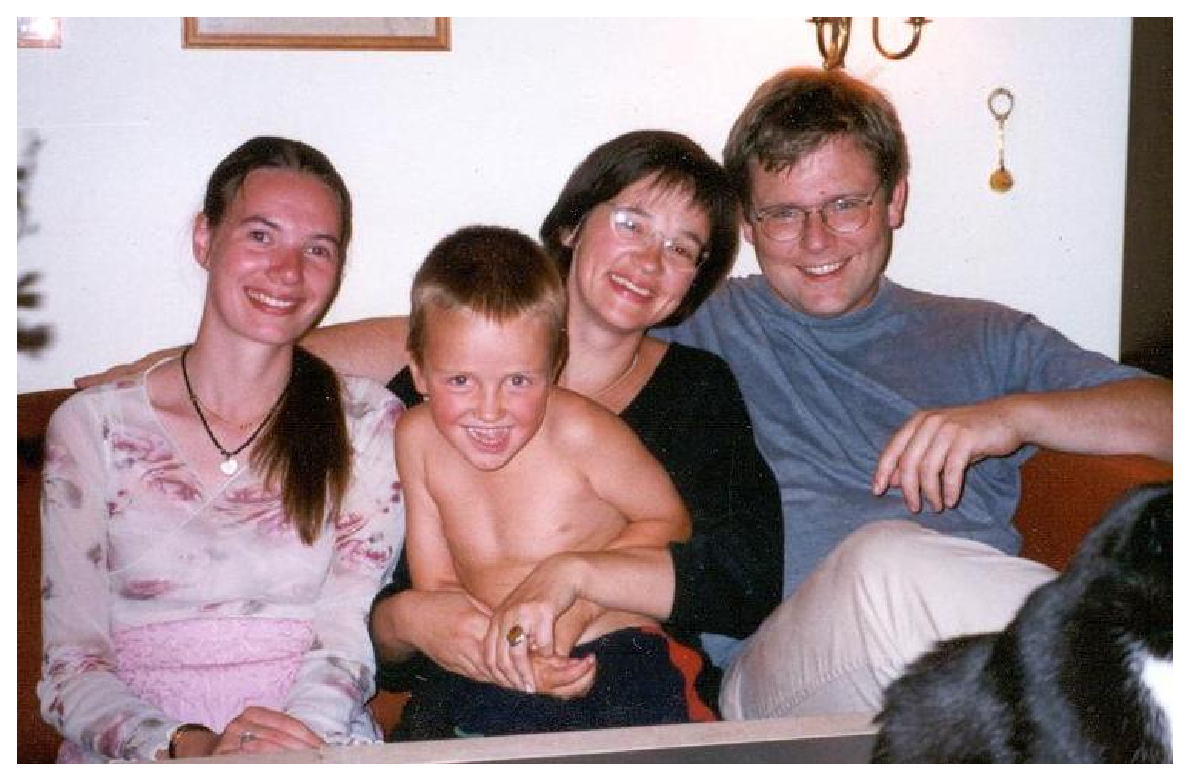
\includegraphics{gr/familie.eps}
\bibliography{books}
\end{document}

%
% and all that was ever heard from him again, was the sound of Tubular Bells! 
%
% %%%%%%%%%%%%%%%%%%%%%%%%%%%%%%%%%%%%%%%%%%%%%%%%%%%%%%%%%%%%%%%%%%%%%%%%%%%
%
% $Log$
% Revision 1.2  2000/03/03 01:27:43  ravn
%
%
% Entered stuff in CVS.  The notes on databases have been added, and the
% section moved to s-sample-databases (me thinks).
%
% Revision 1.1.1.1  2000/03/02 21:55:31  ravn
% Speciale files
%
% Revision 1.6  2000/02/23 02:22:41  ravn
% Moved XML section to seperate file.  Added framepage.
%
% Revision 1.5  2000/02/18 04:31:26  ravn
% Version shipped to immerkaer.
%
% Revision 1.4  2000/02/18 03:14:37  ravn
% Added extra paragraphcs after talking to jimm
%
% Revision 1.3  2000/02/15 18:35:37  ravn
% Updated to include misc notes from MIP file system.
%
% Revision 1.2  2000/02/14 04:52:10  ravn
% Added much more text.  Played with fonts.
%
% Revision 1.1  2000/02/14 02:52:22  ravn
% Initial revision
%
